\section{Introduction}





Inference-time compute has unlocked a new axis for scaling AI capabilities. Recent advancements in Large Reasoning Models (LRMs) such as OpenAI o1/o3~\citep{openai_o1,openai_o3} and DeepSeek R1~\citep{deepseek_r1} have demonstrated state-of-the-art performance across a wide range of complex tasks. 
Although these LRMs share the architectural backbones as traditional large language models (LLMs), their inference behavior differs significantly: LRMs first ``think'' by generating internal {\em thinking} tokens---tokens that decompose a task into a sequence of composable reasoning steps via a long chain-of-thought (CoT)~\citep{cot} before producing the final tokens that summarize the reasoning process.

Despite their promise, LRMs incur substantial inference latency due to the length of the reasoning sequences they generate. This challenge is primarily driven by the autoregressive nature of LLMs, where decoding time scales linearly with sequence length. As a result, final output generation can routinely take minutes, if not hours, to answer a single query; such delays far exceed those of typical LLMs and are prohibitively slow for many interactive applications, ultimately degrading user experience~\citep{certaindex}.

Our approach to tackling reasoning delays---{\bf without compromising accuracy}---is rooted in two fundamental properties of LRMs: (1) LRMs tackle difficult tasks by generating long CoTs that decompose them into many simpler, sequential steps. For example, in mathematical problem solving, a few key reasoning steps require complex long-term planning and have a major influence on downstream reasoning, while most subsequent steps simply execute the plan through straightforward calculations or case analyses (Fig.~\ref{fig:toy_example});
(2) The utility of an individual reasoning step hinges less on the exact wording of the thinking tokens but more on the {\em semantic insight} it provides.
That is,  as long as a step contributes meaningfully to advancing the CoT, it remains effective—even if phrased imprecisely or differently (Fig.~\ref{fig:equiv_spectrum}).
Moreover, LRMs possess self-reflection capabilities that enable them to revise or correct occasional missteps from earlier steps. 

\textbf{Taken together, these properties make the decoding of thinking tokens---the dominant source of inference latency in LRMs---inherently more \emph{approximation tolerant} than typical LLM decoding}. A large fraction of intermediate reasoning steps can be effectively handled by lightweight reasoning models, which both align with the nature of these steps and can tolerate minor inaccuracies. As shown in Fig.~\ref{fig:main_results}, this opens the door to significantly faster inference without sacrificing output quality.




\begin{figure}[t]
    \centering
    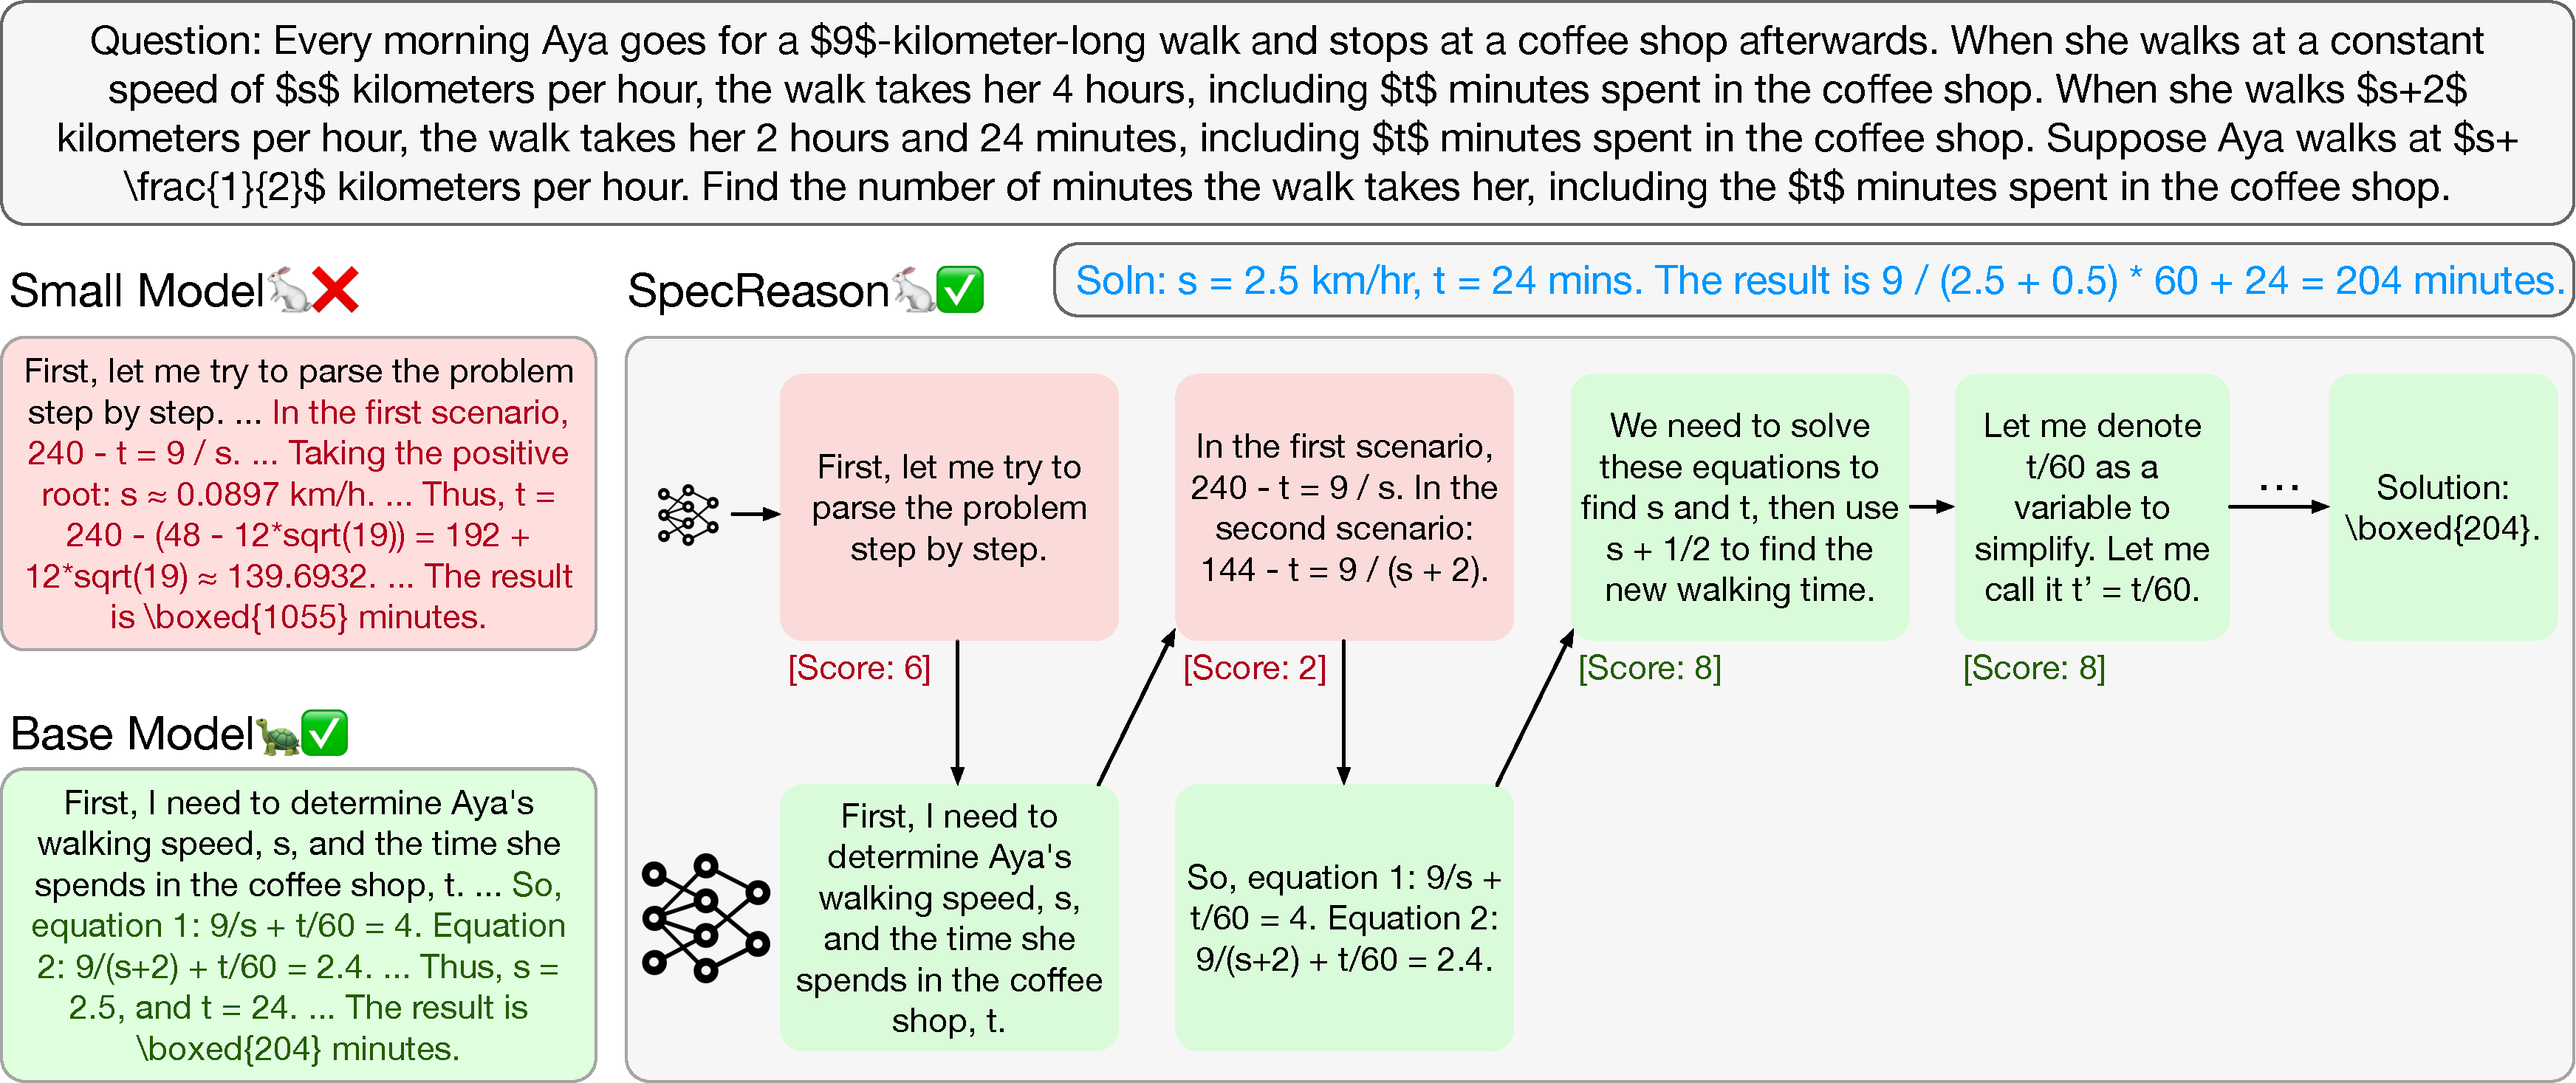
\includegraphics[width=0.99\textwidth]{figures/toy_example.pdf}
    \caption{\name{} leverages a smaller reasoning model to speculate individual reasoning steps, deferring to the base model only for assessment (and optionally as a fallback), enabling faster yet accurate reasoning. For illustration, we show a math question as an example; our evaluation includes more general reasoning workloads.}
    \label{fig:toy_example}
\end{figure}

    
Building on these insights, we propose \textbf{\name{}}, a system for accelerating LRM inference by selectively offloading easier intermediate steps to be {\em speculated} by a smaller model without compromising final output accuracy. 
\name{} employs a lightweight reasoning model to generate individual reasoning steps, while reserving the slower but more capable base model to efficiently verify these speculated steps (\S\ref{sec:spec_reason}) and guide the reasoning process along the correct trajectory (Fig.~\ref{fig:toy_example}). 
Consistent with prior findings~\citep{prmbench}, we observe that base models can be prompted to act as critic models---assessing the utility of intermediate steps and accepting or rejecting them as needed (Fig.~\ref{fig:prm_microbenchmark}). %


\textbf{Speculative reasoning vs. speculative decoding.} While \name{} is conceptually related to speculative decoding~\citep{spec_decoding}, which accelerates LLM inference by using a smaller draft model to predict future tokens, there are key distinctions between the two. Most notably, speculative decoding is an \emph{exact} optimization: it relies on {\em token}-level equivalence between the small and base models, i.e., focusing on typical LLM serving where all generated tokens are part of the final model output being assessed. In contrast, \name{} explicitly leverages the {\em approximation tolerance} inherent in reasoning: it targets {\em thinking tokens}---intermediate steps in the reasoning process---where semantic alignment, rather than token-level equivalence, is sufficient.
This relaxation enables substantial latency savings during LRM inference, as semantically similar intermediate steps (Fig.~\ref{fig:equiv_spectrum}) are often adequate to preserve end-task accuracy (Fig.~\ref{fig:main_results}).
In many cases, \name{} even \emph{improves} final accuracy over the base model by generating fewer unnecessary tokens (Fig.~\ref{fig:acc_intuition}).
To further address the high inference cost of LRMs, \name{} also exposes a user-configurable knob that allows trading off accuracy for latency by adjusting the tolerance level for speculative approximations.
Finally and most importantly, because speculative reasoning and speculative decoding operate at different levels, we show that they are \emph{complementary} techniques (\S\ref{sec:hierarchical_speculation}), and when combined in a hierarchical speculation framework, achieve even greater reductions in inference latency.



We evaluate \name{} across a wide range of reasoning workloads spanning tasks of varying complexity~\citep{aime,math500,gpqa}. Overall, \name{} reduces end-to-end inference latency by $1.4-3.0\times$ compared to vanilla LRM inference while improving accuracy by $0.4-9.0\%$. Moreover, \name{} can be {\em combined} with speculative decoding to provide an additional $8.8-58.0\%$ improvement over speculative decoding alone.





    





